\originalchapter{作业 3}
MIT 18.330, Spring 2012. 原件: Homework 3, Due March 15. 以下解答均为 AI 编写, 非官方答案.

\begin{exercise}\label{ps3-q1}
(原题 1, 2.5 分) 通过对适当的插值多项式求导, 用 $f(0),f(h),f(2h)$ 设计 $f'(0)$ 的单边二阶差分公式; $0$ 是左端点. 用 Taylor 展开或课堂结果证明精度.
\end{exercise}
\begin{solution}
节点 $0,h,2h$ 的二次 Lagrange 插值多项式为
\[
p(x)=f(0)\frac{(x-h)(x-2h)}{2h^2}
-f(h)\frac{x(x-2h)}{h^2}+f(2h)\frac{x(x-h)}{2h^2}.
\]
求导后 $p'(0)=[-3f(0)+4f(h)-f(2h)]/(2h)$. 若 $f\in C^3$, 代入各节点的 Taylor 展开, 常数项及二阶项抵消, 得 $p'(0)=f'(0)-h^2f'''(0)/3+o(h^2)$, 因而是二阶单边公式.
\end{solution}

\begin{exercise}\label{ps3-q2}
(原题 2, 2.5 分) 考虑课堂上的 $[1\ 4\ 1]$ Simpson 公式
$\int_{-h}^h f(x)\dd x\simeq\frac h3[f(-h)+4f(0)+f(h)]$.
\begin{enumerate}[label=(\alph*)]
\item 虽然它由抛物线导出, 证明它对所有三次多项式仍精确.
\item 利用此结论证明, 若 $f\in C^4[-h,h]$, 则该积分的局部误差为 $O(h^5)$.
\end{enumerate}
原件补充: 积分四个节点的三次插值多项式得到另一种称为 $3/8$ 法的公式, 其局部误差也为 $O(h^5)$.
\end{exercise}
\begin{solution}
(a) 只需验证基 $1,x,x^2,x^3$: 公式分别给出 $2h,0,2h^3/3,0$, 与积分相同. 奇次项在对称区间及对称权重下都为零.
(b) 将 $f$ 分解为在 $0$ 处的三次 Taylor 多项式 $P_3$ 与余项 $r$, 若第四阶导数在一个固定邻域内有界, 则 $|r(x)|\le M|x|^4/24$. 公式对 $P_3$ 精确, 故总误差绝对值至多
\[
\int_{-h}^h|r(x)|\dd x+
\frac h3(|r(-h)|+4|r(0)|+|r(h)|)
\le \frac{Mh^5}{60}+\frac{Mh^5}{36}=\frac{2M}{45}h^5.
\]
该界不追求最优常数, 但已证明所需局部阶. 固定区间上的复合 Simpson 需再累计小区间数, 得全局四阶.
\end{solution}

\begin{exercise}\label{ps3-q3}
(原题 3, 2.5 分) 实现两端导数为零的夹持三次样条插值. 节点 $x_j=j$, $0\le j\le N$, 数据为
$y_0=1$, $y_1=0$, $y_k=1$ ($k\ge2$). 取 $N=10$, 在远比 10 个点更细的网格上画 $[x_0,x_{10}]$ 内的样条.
\end{exercise}
\begin{solution}
设 $M_j=s''(j)$. 节点处一阶导数连续及两端夹持条件给出三对角系统
\[
2M_0+M_1=6(y_1-y_0),\quad
M_{j-1}+4M_j+M_{j+1}=6(y_{j+1}-2y_j+y_{j-1}),\quad
M_9+2M_{10}=-6(y_{10}-y_9).
\]
中式取 $1\le j\le9$. 矩阵严格对角占优, 故可唯一解出 $M$. 对 $t=x-j\in[0,1]$,
\[
s_j(x)=\frac{M_j(1-t)^3+M_{j+1}t^3}{6}
+(y_j-M_j/6)(1-t)+(y_{j+1}-M_{j+1}/6)t.
\]
实验脚本显式组装并解该系统, 在 2001 个点上求值. 与 SciPy 的夹持样条独立实现比较, 最大差小于 $10^{-13}$, 两端导数均在舍入误差内为零. 图中的小幅振荡随远离凹陷节点快速衰减.
\begin{center}
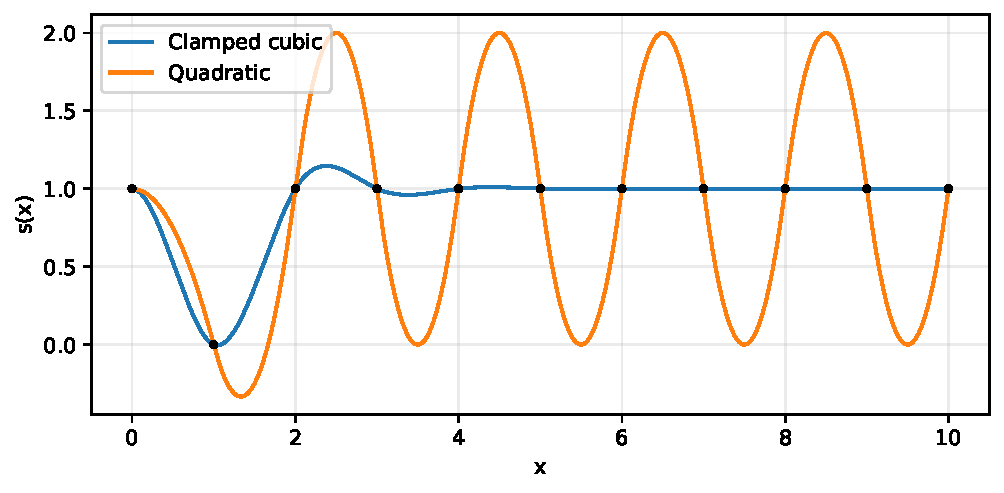
\includegraphics[width=.9\linewidth]{figures/assessments/ps3_splines.pdf}
\end{center}
图中三次样条和下一题的二次样条共用相同数据点与相同坐标轴, 便于比较.
\end{solution}

\begin{exercise}\label{ps3-q4}
(原题 4, 2.5 分) 二次样条是各段为二次多项式、节点处有一个连续导数的插值函数. 对数据 $\{x_j,y_j\}$, 在 $[x_j,x_{j+1}]$ 上为
\[
s_j(x)=y_j+z_j(x-x_j)+\frac{z_{j+1}-z_j}{2(x_{j+1}-x_j)}(x-x_j)^2,
\qquad z_{j+1}=-z_j+2\frac{y_{j+1}-y_j}{x_{j+1}-x_j}.
\]
插值与连续条件留下一个自由度 $z_0$, 以下取 $z_0=0$.
\begin{enumerate}[label=(\alph*)]
\item 对第 3 题数据计算 $z_j$, $1\le j\le10$.
\item 画 $[x_0,x_{10}]$ 上的二次样条.
\item 用一句话解释实际曲线拟合中二次样条为何不如线性和三次样条.
\end{enumerate}
\end{exercise}
\begin{solution}
(a) 依次得到 $(z_1,\ldots,z_{10})=(-2,4,-4,4,-4,4,-4,4,-4,4)$.
(b) 将这些斜率代入题给公式, 图见上一题的 Quadratic 曲线; 自 $j\ge2$ 起所有数据值虽为 $1$, 区间内部仍在 $0$ 与 $2$ 之间交替偏离.
(c) 二次样条的一阶导数连续约束通过 $z_{j+1}=-z_j+2\Delta y_j$ 传递不衰减的交替振荡, 对本类局部扰动既不如线性样条局部、也不如三次样条平滑稳定. 这解释本实验中的实用缺点, 不断言二次样条在每种用途上都较差.
\end{solution}
